\documentclass[twocolumn]{article}
\usepackage{graphicx}
\usepackage{amsmath}
\usepackage{amssymb} %Use of therefore symbol
\usepackage{hyperref}
\usepackage{caption}



\begin{document}
\title{Lab 1: Monte Carlo Methods}
\author{Alex Matheson, Austin Nguyen}
%\affiliation{Department of Physics and Astronomy, University of Calgary, Calgary AB T2N 1N4 Canada}
\date{\today}
\maketitle

\section{Introduction}
Monte Carlo methods are a series of algorithms that take advantage of random processes to solve complicated systems. Many Monte Carlo methods are used to solve problems that are either difficult or impossible to solve analytically. This lab demonstrated a selection of Monte Carlo methods by applying them to simple mathematical and physical problems. Since all Monte Carlo methods rely on randomness, the lab first examined ways of defining randomness and evaluating simple pseudo-random number generators. Sampling and the metropolis algorithm were demonstrated in a simulation of photon transfer through a material. A simple markov chain example involving meteorology was next considered. Lastly, the technique of annealing was used to demonstrate hill climbing and optimization. The examples in this lab showcase a number of Monte Carlo applications, but further applications include climate change simulations, radiation treatment, and financial planning.

\section{Methods}
\subsection{Random Numbers}
Fortran code was written to generate random numbers using a pseudo-random number generator, using input parameters $I_0=3$, $A=7$, $C=0$, and $M=10$. The sequence was shown to repeat, following a pattern of $1,7,9,3,...$ . This pattern is clearly not random, and repeats. The sequence must repeat after at most $M$ entries. Since there are $M$ possible results from the equation, the longest possible sequence generates each number $0=<n<M$ at most once, since once a previous value from the sequence is drawn, the sequence begins to repeat. 

A more elaborate version of this pseudo-random generator was constructed with larger constants. A correlation plot was made to visualize how subsequent values in the sequence were related. Figure \ref{fig:fig1} shows the plot. The result shows that this sequence is not truly random, with some pattern existing between the subsequent numbers. For a 'truly random' sequence, some numbers might be more related than others, and it would be expected that while all numbers did not have the same correlation, at least some would. Another correlation plot, figure \ref{fig:fig2}, shows a different problem. The numbers in the sequence clearly follow a repeating pattern. In pseudo-random generators such as  the example here, the number of random numbers before repition is $n <= M$. In this case, the less than nature is evident. Figure \ref{fig:fig3} shows a plot without such problems. The results in this case appear to have no correlation between $x_n$ and $x_{n+1}$ and are shown similar to random noise. Still, other methods should be used to verify that there is no underlying pattern present. 

\begin{figure}
\centering
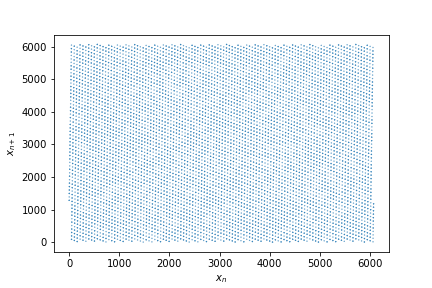
\includegraphics[width=\linewidth]{fig1}
\caption{A correlation plot for a pseudo-random sequence with $A=106$, $C=1283$, and $M=6075$.}
\label{fig:fig1}
\end{figure}

\begin{figure}
	\centering
	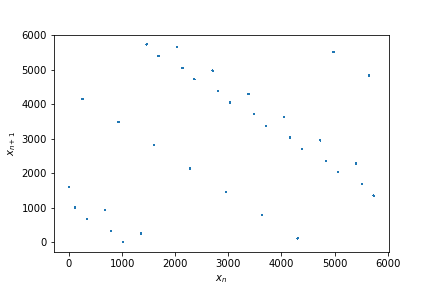
\includegraphics[width=\linewidth]{fig2}
	\caption{A correlation plot for a pseudo-random sequence with $A=107$, $C=1283$, and $M=6075$. Note that this is a change of 1 in variable $A$ from figure \ref{fig:fig2}}
	\label{fig:fig2}
\end{figure}

\begin{figure}
	\centering
	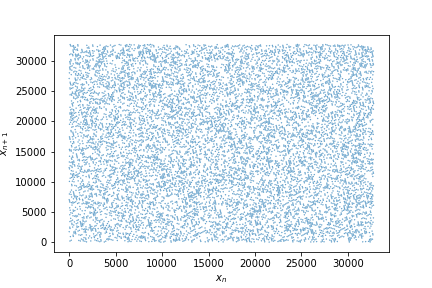
\includegraphics[width=\linewidth]{fig3}
	\caption{A correlation plot for a pseudo-random sequence with $A=1103515245$, $C=12345$, and $M=32768$.}
	\label{fig:fig3}
\end{figure}

Next, the autocorrelation function was examined. A good sequence of random numbers should have a low autocorrelation value. The above pseudo-random generator was tested alongside the gfortran random number generator.

As mentioned above, a correlation plot alone does not determine randomness. Figure \ref{fig:fig4} shows that values previously assumed to be random most certainly are not. When looking at the sequence of numbers generated, the top of the figure clearly shows a repeating pattern present. The autocorrelation function also shows that it takes some time for the function to approach zero. 

The gfortran random number generator was also tested. The sequence of values obtained appears random to the naked eye. The auto-correlation plot also shows an expected decrease toward zero. The value of the auto-correlation function at its peak also is approximately half that of the previous pseudo-random generator. As one would expect, the fortran's inherent generator was constructed better than a single line equation, both in terms of values generated, and auto-correlation.

\begin{figure}
\centering
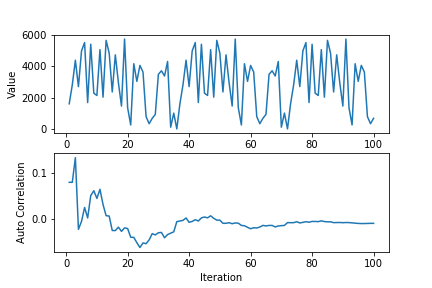
\includegraphics[width=\linewidth]{fig4}
\caption{Random numbers generated by the same pseudo-random generator as figure \ref{fig:fig3}. The top plot shows the numbers generated, while the bottom plot shows the auto-correlation function.}
\label{fig:fig4}
\end{figure}

\begin{figure}
	\centering
	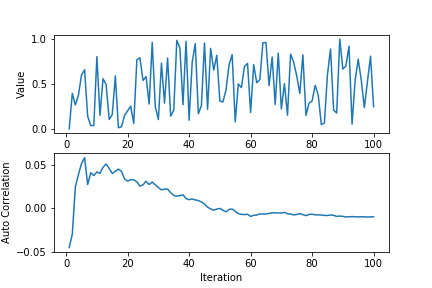
\includegraphics[width=\linewidth]{fig5}
	\caption{Random numbers generated by gfortran's internal RAND() function.}
	\label{fig:fig4}
\end{figure}

\subsection{Light Diffusion}
A number of equations were provided for different parameters in a light diffusion scenario. In this scenario, a photon enters a uniform slab and interacts with matter inside. The possible interactions are absorption, scattering, or exiting the medium. To simulate the path of a single photon through the slab, each parameter in the equations need to be randomly sampled. These parameters are not necessarily uniform. Using the fundamental principle, a sampling equation could be determined. Each probability density was turned into a cumulative probability density, and then inverted. First, a sampling equation for optical depth was determined:

\begin{equation}
\label{eq:tau_sample}
\begin{split}
P(\tau) d\tau =& e^{-\tau} d\tau \\
F_{\tau} (\tau) =& \frac{\int_{0}^{x} e^{-\tau} d\tau}{\int_{0}^{\tau_{max} = 10} e^{-\tau} d\tau}\\
				=& \frac{-e^{-x} + 1}{-e^{-10} + 1}\\
\tau =& F^{-1}_{\tau}(u) \\
\tau =& -ln(1-u(1-e^{-10}))
\end{split}
\end{equation}

Next, the distribution for initial orientation $\theta$ was provided. From this random samples could be determined:
\begin{equation}
\label{eq:theta_sample}
\begin{split}
P(\theta) d\theta =& \frac{1}{2} \sin(\theta) \\
F_{\theta} (\theta) =& \frac{\int_{0}^{x} \frac{1}{2} sin(\theta) d\theta}{\int_{0}^{\pi} \frac{1}{2} sin(\theta) d\theta}\\
					=& \frac{-\cos(x) + 1}{2}\\
\theta =& F^{-1}_{\theta}(u) \\
\theta =& \arccos(1-2u)
\end{split}
\end{equation}

Lastly, angle $\phi$ needed to be considered. Thankfully, this variable was already uniform.

%FIX HERE  HERE  HERE  HERE  HERE

The length travelled through the medium was dependent on the optical depth.
\begin{equation}
\begin{split}
L =& \int_{0}^{\tau_{max}}\sigma n dz \\
\end{split}
\end{equation}

%FIX HERE  HERE  HERE  HERE  HERE

For most of the path of a photon, the exit condition will not be in play. For the rest of the medium, the probability of a photon being scattered is:
\begin{equation}
prob = \frac{P_s}{P_s + P_a}
\end{equation}

This probability has two extreme cases. Since the two probabilities must add together to $1$, the absorb or scatter condition has value $1$ associated with complete scattering (when $P_s = 1$ and $P_a=0$) or value $0$ for complete absorption (when $P_s = 0$ and $P_a=1$).

To test the above distributions, each random number formula was written in fortran and used to generate a series of histograms. If the histograms recreate the original probability densities set out for the variable, the random generator was assumed to be working correctly. Figures \ref{fig:fig6}, \ref{fig:fig7} and \ref{fig:fig8} show $\tau$, $\theta$ and $\phi$ respectively.

\begin{figure}
\centering
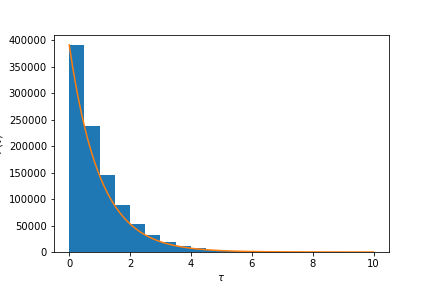
\includegraphics[width=\linewidth]{fig6}
\caption{Histogram for random values of $\tau$ generated by final equation \ref{eq:tau_sample}. The orange curve represents the expected distribution.}
\label{fig:fig6}
\end{figure}

\begin{figure}
\centering
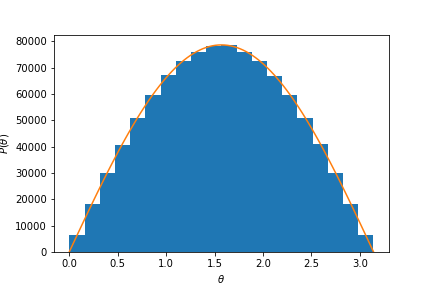
\includegraphics[width=\linewidth]{fig7}
\caption{Histogram for random values of $\theta$ generated by the final equation in set \ref{eq:theta_sample}. The orange curve represents the expected distribution}
\label{fig:fig7}
\end{figure}

\begin{figure}
	\centering
	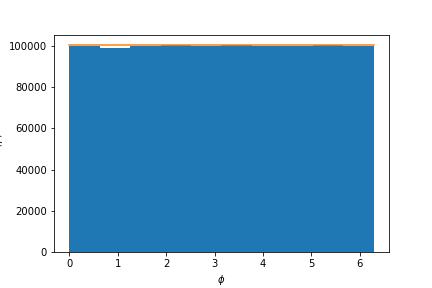
\includegraphics[width=\linewidth]{fig8}
	\caption{Histogram for random values of $\phi$ generated by a uniform random number generator. The orange curve represents the expected distribution.}
	\label{fig:fig8}
\end{figure}

\subsection{Annealing}
In an annealing procedure, the acceptance probability of completing a change after a proposed step forward is modified by a temperature $T$. The acceptance is now defined as:
$A(x_n \to x^*) = Min \Bigg( 1, \Big( \frac{P(x^*)}{P(x_n)}\Big) ^{ \frac{1}{T(n)} } \Bigg)$
When $T=1$, the algorithm that is recovered is a simple metropolis algorithm. 

In a hyporthetical scenario, the probability term is set to 0.5 and $T=100$ initially, yielding acceptance of $0.93$. After some time, $T=1$ and the acceptance reduces to $0.5$. After still more time, $T=0.1$ and the acceptance is $0.000977$. Because of the inverse nature of $T$ in the exponent, a reduction in $T$ makes a change exponentially less likely to occur. This is typically desirable when using annealing. Ideally, the random walker being used by the algorithm is able to escape local maxima and jump to other peaks in the region early on. As time goes on, the algorithm should lower the acceptance so that it hones in on the actual peak.

%Seek clarification on e^-E question

\section{Discussion}


\section{Conclusion}

\begin{thebibliography}{00}
	\bibitem{ouyed}
	Ouyed and Dobler, PHYS 581 course notes, Department of Physics and Astrophysics, University of Calgary (2016).
	\bibitem{NR}
	W. Press et al., \emph{Numerical Recipes} (Cambridge University Press, 2010) 2nd. Ed.
\end{thebibliography}

\section{Appendix}

	
\end{document}